\chapter{Experiments and Results}

This should most likely contain both the results from the classification task and the visualization task.

\textcolor{blue}{(8-10 pages) In this chapter you present your results from your work, coming from 
testing/validating/exploring the theory/research-questions by empirical studies. It can be structured by contributions, 
research questions, or studies done. Find what suits your thesis and results. Some also like to include the 
bibliography of the included papers with abstract and identified contributions towards the thesis. Do not use all of 
the headlines below, if it leads to the same point being said over and over. Find the approach that best makes your 
point.}

\begin{figure}[htb]
 \begin{center}
     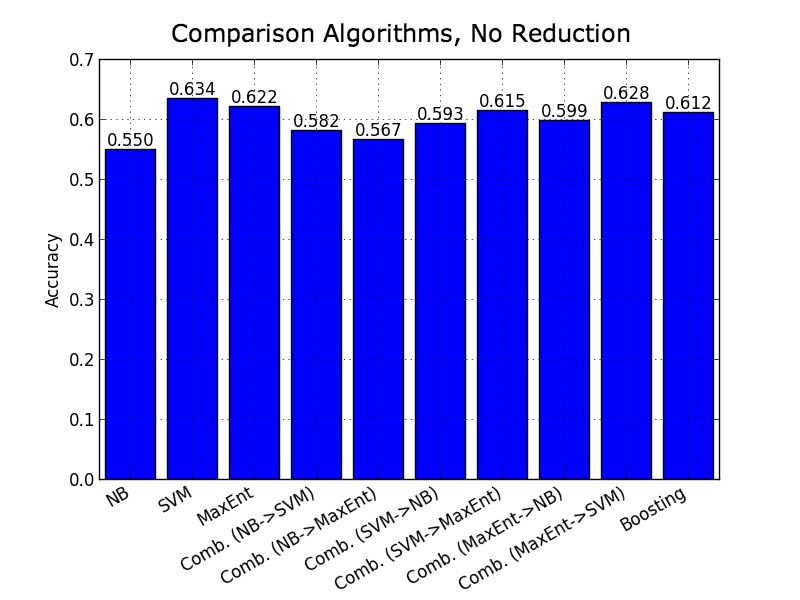
\includegraphics[width=1.\textwidth]{../img/plots/comparison_no_reduce.png}
 \end{center}
 \caption[Comparison of different algorithms with a dateset without reduction]{Show accuracy of the different algorithms when not normalizing the number of entires per class in the development set.}
 \label{plot:comparison_no_reduce}
\end{figure}





\textcolor{green}{Summary of the studies Study 1: \ldots StudyN)}

\textcolor{green}{Overview of the contributions Contribution C1: \ldots CN}

\textcolor{green}{Research questions answered RQ1: \ldots RQN}

\textcolor{green}{Paper Abstracts P1 \ldots PN}